%% bare_conf.tex
%% V1.3
%% 2007/01/11
%% by Michael Shell
%% See:
%% http://www.michaelshell.org/
%% for current contact information.
%%
%% This is a skeleton file demonstrating the use of IEEEtran.cls
%% (requires IEEEtran.cls version 1.7 or later) with an IEEE conference paper.
%%
%% Support sites:
%% http://www.michaelshell.org/tex/ieeetran/
%% http://www.ctan.org/tex-archive/macros/latex/contrib/IEEEtran/
%% and
%% http://www.ieee.org/

%%*************************************************************************
%% Legal Notice:
%% This code is offered as-is without any warranty either expressed or
%% implied; without even the implied warranty of MERCHANTABILITY or
%% FITNESS FOR A PARTICULAR PURPOSE! 
%% User assumes all risk.
%% In no event shall IEEE or any contributor to this code be liable for
%% any damages or losses, including, but not limited to, incidental,
%% consequential, or any other damages, resulting from the use or misuse
%% of any information contained here.
%%
%% All comments are the opinions of their respective authors and are not
%% necessarily endorsed by the IEEE.
%%
%% This work is distributed under the LaTeX Project Public License (LPPL)
%% ( http://www.latex-project.org/ ) version 1.3, and may be freely used,
%% distributed and modified. A copy of the LPPL, version 1.3, is included
%% in the base LaTeX documentation of all distributions of LaTeX released
%% 2003/12/01 or later.
%% Retain all contribution notices and credits.
%% ** Modified files should be clearly indicated as such, including  **
%% ** renaming them and changing author support contact information. **
%%
%% File list of work: IEEEtran.cls, IEEEtran_HOWTO.pdf, bare_adv.tex,
%%                    bare_conf.tex, bare_jrnl.tex, bare_jrnl_compsoc.tex
%%*************************************************************************

% *** Authors should verify (and, if needed, correct) their LaTeX system  ***
% *** with the testflow diagnostic prior to trusting their LaTeX platform ***
% *** with production work. IEEE's font choices can trigger bugs that do  ***
% *** not appear when using other class files.                            ***
% The testflow support page is at:
% http://www.michaelshell.org/tex/testflow/



% Note that the a4paper option is mainly intended so that authors in
% countries using A4 can easily print to A4 and see how their papers will
% look in print - the typesetting of the document will not typically be
% affected with changes in paper size (but the bottom and side margins will).
% Use the testflow package mentioned above to verify correct handling of
% both paper sizes by the user's LaTeX system.
%
% Also note that the "draftcls" or "draftclsnofoot", not "draft", option
% should be used if it is desired that the figures are to be displayed in
% draft mode.
%
\documentclass[10pt, conference, compsocconf]{IEEEtran}
% Add the compsocconf option for Computer Society conferences.
%
% If IEEEtran.cls has not been installed into the LaTeX system files,
% manually specify the path to it like:
% \documentclass[conference]{../sty/IEEEtran}





% Some very useful LaTeX packages include:
% (uncomment the ones you want to load)


% *** MISC UTILITY PACKAGES ***
%
%\usepackage{ifpdf}
% Heiko Oberdiek's ifpdf.sty is very useful if you need conditional
% compilation based on whether the output is pdf or dvi.
% usage:
% \ifpdf
%   % pdf code
% \else
%   % dvi code
% \fi
% The latest version of ifpdf.sty can be obtained from:
% http://www.ctan.org/tex-archive/macros/latex/contrib/oberdiek/
% Also, note that IEEEtran.cls V1.7 and later provides a builtin
% \ifCLASSINFOpdf conditional that works the same way.
% When switching from latex to pdflatex and vice-versa, the compiler may
% have to be run twice to clear warning/error messages.






% *** CITATION PACKAGES ***
%
\usepackage{cite}
% cite.sty was written by Donald Arseneau
% V1.6 and later of IEEEtran pre-defines the format of the cite.sty package
% \cite{} output to follow that of IEEE. Loading the cite package will
% result in citation numbers being automatically sorted and properly
% "compressed/ranged". e.g., [1], [9], [2], [7], [5], [6] without using
% cite.sty will become [1], [2], [5]--[7], [9] using cite.sty. cite.sty's
% \cite will automatically add leading space, if needed. Use cite.sty's
% noadjust option (cite.sty V3.8 and later) if you want to turn this off.
% cite.sty is already installed on most LaTeX systems. Be sure and use
% version 4.0 (2003-05-27) and later if using hyperref.sty. cite.sty does
% not currently provide for hyperlinked citations.
% The latest version can be obtained at:
% http://www.ctan.org/tex-archive/macros/latex/contrib/cite/
% The documentation is contained in the cite.sty file itself.






% *** GRAPHICS RELATED PACKAGES ***
%
\ifCLASSINFOpdf
  \usepackage[pdftex]{graphicx}
  % declare the path(s) where your graphic files are
  % \graphicspath{{../pdf/}{../jpeg/}}
  % and their extensions so you won't have to specify these with
  % every instance of \includegraphics
  \DeclareGraphicsExtensions{.pdf,.jpeg,.png}
\else
  % or other class option (dvipsone, dvipdf, if not using dvips). graphicx
  % will default to the driver specified in the system graphics.cfg if no
  % driver is specified.
  \usepackage[dvipdfm]{graphicx}
  % declare the path(s) where your graphic files are
  % \graphicspath{{../eps/}}
  % and their extensions so you won't have to specify these with
  % every instance of \includegraphics
  \DeclareGraphicsExtensions{.eps}
\fi
% graphicx was written by David Carlisle and Sebastian Rahtz. It is
% required if you want graphics, photos, etc. graphicx.sty is already
% installed on most LaTeX systems. The latest version and documentation can
% be obtained at: 
% http://www.ctan.org/tex-archive/macros/latex/required/graphics/
% Another good source of documentation is "Using Imported Graphics in
% LaTeX2e" by Keith Reckdahl which can be found as epslatex.ps or
% epslatex.pdf at: http://www.ctan.org/tex-archive/info/
%
% latex, and pdflatex in dvi mode, support graphics in encapsulated
% postscript (.eps) format. pdflatex in pdf mode supports graphics
% in .pdf, .jpeg, .png and .mps (metapost) formats. Users should ensure
% that all non-photo figures use a vector format (.eps, .pdf, .mps) and
% not a bitmapped formats (.jpeg, .png). IEEE frowns on bitmapped formats
% which can result in "jaggedy"/blurry rendering of lines and letters as
% well as large increases in file sizes.
%
% You can find documentation about the pdfTeX application at:
% http://www.tug.org/applications/pdftex





% *** MATH PACKAGES ***
%
%\usepackage[cmex10]{amsmath}
% A popular package from the American Mathematical Society that provides
% many useful and powerful commands for dealing with mathematics. If using
% it, be sure to load this package with the cmex10 option to ensure that
% only type 1 fonts will utilized at all point sizes. Without this option,
% it is possible that some math symbols, particularly those within
% footnotes, will be rendered in bitmap form which will result in a
% document that can not be IEEE Xplore compliant!
%
% Also, note that the amsmath package sets \interdisplaylinepenalty to 10000
% thus preventing page breaks from occurring within multiline equations. Use:
%\interdisplaylinepenalty=2500
% after loading amsmath to restore such page breaks as IEEEtran.cls normally
% does. amsmath.sty is already installed on most LaTeX systems. The latest
% version and documentation can be obtained at:
% http://www.ctan.org/tex-archive/macros/latex/required/amslatex/math/





% *** SPECIALIZED LIST PACKAGES ***
%
%\usepackage{algorithmic}
% algorithmic.sty was written by Peter Williams and Rogerio Brito.
% This package provides an algorithmic environment fo describing algorithms.
% You can use the algorithmic environment in-text or within a figure
% environment to provide for a floating algorithm. Do NOT use the algorithm
% floating environment provided by algorithm.sty (by the same authors) or
% algorithm2e.sty (by Christophe Fiorio) as IEEE does not use dedicated
% algorithm float types and packages that provide these will not provide
% correct IEEE style captions. The latest version and documentation of
% algorithmic.sty can be obtained at:
% http://www.ctan.org/tex-archive/macros/latex/contrib/algorithms/
% There is also a support site at:
% http://algorithms.berlios.de/index.html
% Also of interest may be the (relatively newer and more customizable)
% algorithmicx.sty package by Szasz Janos:
% http://www.ctan.org/tex-archive/macros/latex/contrib/algorithmicx/




% *** ALIGNMENT PACKAGES ***
%
%\usepackage{array}
% Frank Mittelbach's and David Carlisle's array.sty patches and improves
% the standard LaTeX2e array and tabular environments to provide better
% appearance and additional user controls. As the default LaTeX2e table
% generation code is lacking to the point of almost being broken with
% respect to the quality of the end results, all users are strongly
% advised to use an enhanced (at the very least that provided by array.sty)
% set of table tools. array.sty is already installed on most systems. The
% latest version and documentation can be obtained at:
% http://www.ctan.org/tex-archive/macros/latex/required/tools/


%\usepackage{mdwmath}
%\usepackage{mdwtab}
% Also highly recommended is Mark Wooding's extremely powerful MDW tools,
% especially mdwmath.sty and mdwtab.sty which are used to format equations
% and tables, respectively. The MDWtools set is already installed on most
% LaTeX systems. The lastest version and documentation is available at:
% http://www.ctan.org/tex-archive/macros/latex/contrib/mdwtools/


% IEEEtran contains the IEEEeqnarray family of commands that can be used to
% generate multiline equations as well as matrices, tables, etc., of high
% quality.


%\usepackage{eqparbox}
% Also of notable interest is Scott Pakin's eqparbox package for creating
% (automatically sized) equal width boxes - aka "natural width parboxes".
% Available at:
% http://www.ctan.org/tex-archive/macros/latex/contrib/eqparbox/





% *** SUBFIGURE PACKAGES ***
%\usepackage[tight,footnotesize]{subfigure}
% subfigure.sty was written by Steven Douglas Cochran. This package makes it
% easy to put subfigures in your figures. e.g., "Figure 1a and 1b". For IEEE
% work, it is a good idea to load it with the tight package option to reduce
% the amount of white space around the subfigures. subfigure.sty is already
% installed on most LaTeX systems. The latest version and documentation can
% be obtained at:
% http://www.ctan.org/tex-archive/obsolete/macros/latex/contrib/subfigure/
% subfigure.sty has been superceeded by subfig.sty.



%\usepackage[caption=false]{caption}
%\usepackage[font=footnotesize]{subfig}
% subfig.sty, also written by Steven Douglas Cochran, is the modern
% replacement for subfigure.sty. However, subfig.sty requires and
% automatically loads Axel Sommerfeldt's caption.sty which will override
% IEEEtran.cls handling of captions and this will result in nonIEEE style
% figure/table captions. To prevent this problem, be sure and preload
% caption.sty with its "caption=false" package option. This is will preserve
% IEEEtran.cls handing of captions. Version 1.3 (2005/06/28) and later 
% (recommended due to many improvements over 1.2) of subfig.sty supports
% the caption=false option directly:
%\usepackage[caption=false,font=footnotesize]{subfig}
%
% The latest version and documentation can be obtained at:
% http://www.ctan.org/tex-archive/macros/latex/contrib/subfig/
% The latest version and documentation of caption.sty can be obtained at:
% http://www.ctan.org/tex-archive/macros/latex/contrib/caption/




% *** FLOAT PACKAGES ***
%
%\usepackage{fixltx2e}
% fixltx2e, the successor to the earlier fix2col.sty, was written by
% Frank Mittelbach and David Carlisle. This package corrects a few problems
% in the LaTeX2e kernel, the most notable of which is that in current
% LaTeX2e releases, the ordering of single and double column floats is not
% guaranteed to be preserved. Thus, an unpatched LaTeX2e can allow a
% single column figure to be placed prior to an earlier double column
% figure. The latest version and documentation can be found at:
% http://www.ctan.org/tex-archive/macros/latex/base/



%\usepackage{stfloats}
% stfloats.sty was written by Sigitas Tolusis. This package gives LaTeX2e
% the ability to do double column floats at the bottom of the page as well
% as the top. (e.g., "\begin{figure*}[!b]" is not normally possible in
% LaTeX2e). It also provides a command:
%\fnbelowfloat
% to enable the placement of footnotes below bottom floats (the standard
% LaTeX2e kernel puts them above bottom floats). This is an invasive package
% which rewrites many portions of the LaTeX2e float routines. It may not work
% with other packages that modify the LaTeX2e float routines. The latest
% version and documentation can be obtained at:
% http://www.ctan.org/tex-archive/macros/latex/contrib/sttools/
% Documentation is contained in the stfloats.sty comments as well as in the
% presfull.pdf file. Do not use the stfloats baselinefloat ability as IEEE
% does not allow \baselineskip to stretch. Authors submitting work to the
% IEEE should note that IEEE rarely uses double column equations and
% that authors should try to avoid such use. Do not be tempted to use the
% cuted.sty or midfloat.sty packages (also by Sigitas Tolusis) as IEEE does
% not format its papers in such ways.





% *** PDF, URL AND HYPERLINK PACKAGES ***
%
\usepackage{url}
% url.sty was written by Donald Arseneau. It provides better support for
% handling and breaking URLs. url.sty is already installed on most LaTeX
% systems. The latest version can be obtained at:
% http://www.ctan.org/tex-archive/macros/latex/contrib/misc/
% Read the url.sty source comments for usage information. Basically,
% \url{my_url_here}.





% *** Do not adjust lengths that control margins, column widths, etc. ***
% *** Do not use packages that alter fonts (such as pslatex).         ***
% There should be no need to do such things with IEEEtran.cls V1.6 and later.
% (Unless specifically asked to do so by the journal or conference you plan
% to submit to, of course. )


% correct bad hyphenation here
\hyphenation{op-tical net-works semi-conduc-tor}


\begin{document}
%
% paper title
% can use linebreaks \\ within to get better formatting as desired
\title{A weighted image reconstruction based on PCA for pedestrian detection}

%------------------------------------------------------------------------- 
% change the % on next lines to produce the final camera-ready version 
\newif\iffinal
% \finalfalse
\finaltrue
\newcommand{\jemsid}{99999}
%------------------------------------------------------------------------- 

% author names and affiliations
% use a multiple column layout for up to two different
% affiliations

\iffinal
  \author{
     \IEEEauthorblockN{Guilherme V. Carvalho, Lailson B. Moraes, George D. C. Cavalcanti, Tsang I. R.}
     \IEEEauthorblockA{Centro de Inform\'{a}tica (CIn)\\
      Universidade Federal de Pernambuco (UFPE)\\
      Recife, Pernambuco, Brasil\\
      \texttt{\url{http://cin.ufpe.br/~viisar}}\\
      \texttt{\url{{gvc,lbm4,gdcc,tir}@cin.ufpe.br}}}
      
    }
\else
  \author{Sibgrapi paper ID: \jemsid \\ }
\fi

% conference papers do not typically use \thanks and this command
% is locked out in conference mode. If really needed, such as for
% the acknowledgment of grants, issue a \IEEEoverridecommandlockouts
% after \documentclass

% for over three affiliations, or if they all won't fit within the width
% of the page, use this alternative format:
% 
%\author{\IEEEauthorblockN{Michael Shell\IEEEauthorrefmark{1},
%Homer Simpson\IEEEauthorrefmark{2},
%James Kirk\IEEEauthorrefmark{3}, 
%Montgomery Scott\IEEEauthorrefmark{3} and
%Eldon Tyrell\IEEEauthorrefmark{4}}
%\IEEEauthorblockA{\IEEEauthorrefmark{1}School of Electrical and Computer Engineering\\
%Georgia Institute of Technology,
%Atlanta, Georgia 30332--0250\\ Email: see http://www.michaelshell.org/contact.html}
%\IEEEauthorblockA{\IEEEauthorrefmark{2}Twentieth Century Fox, Springfield, USA\\
%Email: homer@thesimpsons.com}
%\IEEEauthorblockA{\IEEEauthorrefmark{3}Starfleet Academy, San Francisco, California 96678-2391\\
%Telephone: (800) 555--1212, Fax: (888) 555--1212}
%\IEEEauthorblockA{\IEEEauthorrefmark{4}Tyrell Inc., 123 Replicant Street, Los Angeles, California 90210--4321}}




% use for special paper notices
%\IEEEspecialpapernotice{(Invited Paper)}


%------------------------------------------------------------------------- 
% Special Sibgrapi teaser
% \teaser{%
%   
\includegraphics[width=.8\linewidth]{teaser}
%   \caption{Overview of our method:\ldots{}}
%   \label{fig:teaser}
% }
%------------------------------------------------------------------------- 



% make the title area
\maketitle


\begin{abstract}
Pedestrian detection is a task associated with security and surveillance systems. Its inherently complex nature makes it a hard challenge to develop a detection system. In this article we present an analysis of a pedestrian detection model based on PCA reconstruction errors. We find out that some components of the original classifier are not strictly necessary and can be eliminated to reduce the detection times. We then propose a weighted version of the classifier, that achieves a better classification accuracy.
\end{abstract}

\begin{IEEEkeywords}
pedestrian detection; pattern recognition; principal component analysis
\end{IEEEkeywords}


% For peer review papers, you can put extra information on the cover
% page as needed:
% \ifCLASSOPTIONpeerreview
% \begin{center} \bfseries EDICS Category: 3-BBND \end{center}
% \fi
%
% For peerreview papers, this IEEEtran command inserts a page break and
% creates the second title. It will be ignored for other modes.
\IEEEpeerreviewmaketitle



\section{Introduction}
% Discuss about PCA, how it works, PCA for compression, image reconstruction
% Principal Component Analysis (PCA) is currently a commonly used technique in computer vision, specially for dimensionality reduction and feature extraction \cite{}. 

% Still part of description
% Borja et. al. \cite{borja09} uses PCA for... The rationale is that PCA can compress optimally only the kind of images that were used to compute the analysis, and that any other kind of image will not be compressed well using few attributes \cite{borja09}. So, when we compress an image with PCA and reconstruct it, the difference between the original image and the reconstructed one will be small if the image is similar to the images used to do the PCA and correspondingly greater if the image is different. This difference is referred to as \emph{reconstruction error}.

% Cite what components are used
% Mention the word component
% Borja... describe a two-class image classifier that is based on reconstruction error. The classifier is used for object detection, that is, it determines if a given image contains or not contains some kind of object. In other terms, it determines if the image belongs to the positive or to the negative class. To do this, it first perform PCA for positive and negative examples separately. When a new pattern needs to be classified, it is projected on the PCA spaces and subsequently reconstructed. Then, the classifier uses the reconstruction errors to determine the class the pattern belongs to.

Pedestrian detection systems have been widely used and developed throughout the computer vision history. Ranging from still image detection to automated car breaking systems, it is becoming an usual task in our lives.

In this paper we describe a pedestrian detection proposed by Malang\'{o}n-Borja and Fuentes \cite{borja09}. It classifies an image based on how much its reconstruction is different from the original one, that is, it classifies based on the image reconstruction error. We analyze how it works and how its original performance can be improved. The proposed improvements enhances the system's accuracy using weights on the detection errors and significantly reduces execution times by decreasing the number of calculations made by the algorithm.

% In this paper we describe a pedestrian detection model proposed by Malag\'{o}n-Borja and Fuentes \cite{borja09}. It classifies an image based on how much its reconstruction is different from the original one; in other words, based on the image reconstruction error. We analyze how it works and how its original performance can be improved, as well as its detection times, by using weights on the reconstruction errors and reducing the number of calculations made by the algorithm, respectively.

This paper is divided as follows. Section 2 describes an image reconstruction technique using PCA. Section 3 describes how to use image reconstruction to classify images. Section 4 presents our experiments and discussions. Finally, in Section 5 conclusions are presented.


\section{Image reconstruction with PCA}

The idea of principal component analysis (PCA) seems to have been first proposed in 1901 \cite{sirovich87} and was later developed in many works during the last century. It was popularized in computer vision by the eigenfaces method \cite{turk91}, a face recognition model still relevant and used in current days.

Given a set of samples, PCA yields a set of orthonormal vectors that can be used to linearly project the samples into a new space. This space maximizes the projected samples variance and minimizes their least mean square error, that is, it minimizes the difference between the projected sample and its reconstruction back to the original space \cite{shlens09}. This characteristic makes PCA suitable for data compression and dimensionality reduction. The data can come from many kinds of sources, but in this work we are concerned only with images.

The formulation of PCA is as follows. Consider a set of $m$ images, each with $r$ pixels of width and $c$ pixels of height (i.e. of size $r \times c$ pixels). Each image $I_i$ is represented by a column vector $v_i$ of length $rc$. The set mean $\mu$ and the covariance matrix $C$ are given by

\begin{equation}
  \mu = \frac{1}{m} \sum_{i=1}^m{v_i}
\end{equation}

\begin{equation}
  C = \sum_{i=1}^m{(v_i - \mu)(v_i - \mu)^T}.
\end{equation}

PCA applies eigen-decomposition on $C$ and keeps the $k$ eigenvectors ($1 \leq k \leq rc$) corresponding to the $k$ largest eigenvalues. These eigenvectors are called the \emph{principal components} (PCs) of $C$. It is proven that a projection onto the space defined by these eigenvectors provides the optimal reduced representation of the data, minimizing information loss \cite{shlens09}.

Let $P$ be the matrix whose columns are the first $k$ principal components of $C$. The projection $p$ of an image $u$ into this eigenspace is given by

\begin{equation}
  p = P^T (u - \mu).
\end{equation}

\noindent As the projection is reversible, we can recover the original version of a previously projected image. The \emph{reconstructed image} $u'$ of a projection $p$ is

\begin{equation}
  u' = Pp + \mu = PP^T(u - \mu) + \mu.
\end{equation}

\noindent This process can be interpreted as a form of lossy compression and decompression: the reconstructed image is generally not equal to the original one, being just an approximation of it. For this reason, each reconstruction has an associated \emph{reconstruction error}, which can be measured by

\begin{equation}
  d = |u - u'| = \sqrt{\sum{(u_i - u'_i)^2}}.
\end{equation}

The more principal components we use to obtain a projection, the less information loss we have, what allows a more accurate reconstruction. Also, the more similar $u$ is to the images that were used to produce $P$, the better the reconstruction should be for a fixed number of eigenvectors.


\section{Classification using reconstruction}

By definition, PCA looks for the set of PCs that best describe the distribution of the data being analyzed. Therefore, these PCs are going to preserve better the information of the images from which PCA was performed, or of those that are similar to them \cite{borja09}. For example, consider a set of PCs obtained only from images that contains pedestrians. They must reconstruct better images of other pedestrians than any other type of images. Conversely, if we have a set of PCs obtained from images of anything except pedestrians, the reconstruction of pedestrian images must be poor.

Based on this fact, Malag'{o}n-Borja and Fuentes \cite{borja09} proposed a classifier for pedestrian detection that uses reconstruction errors as the classification criteria. In addition to the grayscale images, the classifier also uses the corresponding computed edge images, since they characterize better the pedestrian silhouette and eliminate background and clothing variations. 

In the training phase, PCA must be performed separately for four sets of images, what results in the following sets of PCs:

\begin{itemize}
	\item The principal components $P_{gp}$ and the mean $\mu_{gp}$ from the set of pedestrian grayscale images;
	\item The principal components $P_{ep}$ and the mean $\mu_{ep}$ from the set of pedestrian edge images;
	\item The principal components $P_{gn}$ and the mean $\mu_{gn}$ from the set of non-pedestrian grayscale images;
	\item The principal components $P_{en}$ and the mean $\mu_{en}$ from the set of non-pedestrian edge images.
\end{itemize}

In the classification phase, when a new grayscale image has to be classified, the first step is to obtain its edge image and perform four reconstructions: one for each set of PCs. Then, the reconstruction errors must be calculated and combined to produce the total reconstruction error, that is the final classification score. If the total error is greater than or equal to zero, the image is classified as a pedestrian; otherwise, it is classifier as a non-pedestrian. The detailed procedure is described below.

\begin{enumerate}
  \item Obtain the edge image $e$ from grayscale image $g$ using the Sobel operator;
  \item Perform four image reconstructions:
    \begin{enumerate}
      \item $r_{gp} = P_{gp} P_{gp}^T(g-u) + \mu_{gp}$
      \item $r_{ep} = P_{ep} P_{ep}^T(e-u) + \mu_{ep}$
      \item $r_{gn} = P_{gn} P_{gn}^T(g-u) + \mu_{gn}$
      \item $r_{en} = P_{en} P_{en}^T(e-u) + \mu_{en}$
    \end{enumerate}
  \item Calculate the corresponding reconstruction errors:
    \begin{enumerate}
      \item $d_{gp} = |r_{gp} - g|$
      \item $d_{ep} = |r_{ep} - e|$
      \item $d_{gn} = |r_{gp} - g|$
      \item $d_{en} = |r_{en} - e|$
    \end{enumerate}
  \item Compute the \emph{total reconstruction error}, given by
    \begin{equation}
      d_t = d_{gn} + d_{en} - d_{gp} - d_{ep}
      \label{total_error}
    \end{equation}
  \item Classify the image according to:
    \begin{equation}
      \textrm{class}(g) = \left\{
        \begin{array}{l l}
         \textrm{Pedestrian}, & d_t \geq 0\\
         \textrm{Non-pedestrian}, & d_t < 0
				 \label{classification_score}
        \end{array}
      \right.
    \end{equation}
  
\end{enumerate}

When we analyze how this classifier works, it is easy to understand the role of the PCs generated by the positive samples. As the samples contains the recurrent pattern of the target object (pedestrians in this case), PCA is able to capture it and better reconstruct similar images, generating smaller reconstruction errors. On the other hand, the role of negative PCs is not so clear. Since the negative images contain just random objects and does not represent a specific concept, what pattern is there to capture? We initially thought that the errors of reconstructions obtained from the negative PCs had a negligible importance and therefore it would be possible to eliminate them without impacting the classification accuracy. However, our experiments show that is not the case: it turns out that these errors have a major importance on classification.

We found that the value of the negative PCs is not on the pattern PCA captures, but instead it lies on what pattern it does \emph{not} capture. In this way, the negative reconstruction errors tend to be high for images that contains the target object while for the same images the positive reconstruction errors tend to be small, contributing to a high total error, what classifies the image correctly. For images that does not contains the target object, it is exactly the opposite. Thus, both components of total error (from positive PCs and from negative PCs) work together for classification and that is why it is not worth to construct a classifier that uses only positive reconstruction errors.

However, this does not mean that all the four components have the same relevance to classification. In the reconstruction error classifier, each component contributes equally to the total error, but our experiments show that this relation is not true. Some components have more importance than others and therefore have to be adjusted accordingly. Thus, we propose the \emph{weighted total reconstruction error}, given by

\begin{equation}
  d_w = w_{gn} d_{gn} + w_{en} d_{en} - w_{gp} d_{gp} - w_{ep} d_{ep}
  \label{weighted_total_error}
\end{equation}

\noindent where $w_{gn}$, $w_{en}$, $w_{gp}$, $w_{ep}$ are weights that adjust the relevance of each error to the classification (more relevant errors should have larger weights). They can be set manually or be determined by some optimization algorithm in relation to the training set.

It is also worth noting that the classifier can be made more flexible if we introduce a threshold parameter and compare the classification score (i.e. the total error) agains it, instead of keep it always fixed to zero (as shown in eq.~\ref{classification_score}). In this way, the users can adjust the specificity, depending on their particular application.


\section{Experiments}

The classifier was tested in the context of the pedestrian detection task, that is, given an unlabeled image, the classifier must determine if it depicts or not a pedestrian. To train the classifier, we need a set of pedestrians images and a set of non-pedestrian images. This training phase consists of computing image edges and applying PCA to the four image sets separately, what produces four sets of PCs. They are used to perform the reconstructions on classification time.

The pedestrian images were obtained from the MIT CBCL pedestrian database \cite{cbcl}. It contains 924 color images of pedestrians in frontal or rear views, under different scene conditions. These images were converted to grayscale and had part of the background cropped on the border. The final samples had $45 \times 105$ pixels. This reduces the non-relevant background variation among the images.

The non-pedestrian images were extracted from 120 assorted pictures that did not contain pedestrians. Each one was chopped into slices of $45 \times 105$ pixels and 5.000 slices were randomly chosen to compose the negative dataset. This dataset is more than four times larger than the positive dataset; that is related with the representation capacity of each one. The object detection problem is naturally asymmetric \cite{jiang09}, since the positive examples represents a specific type of object while the negative examples represent the ``rest of the world''. That is why we need more negative examples than positive ones.

To train the classifier, we selected 75\% of the pedestrian images (693 samples) and the remaining images (231 samples) were used  for testing. From the non-pedestrian images, we selected 80\% of the images (4.000 samples) for training the classifier and the remaining images (1.000 samples) were used for testing. This particular scheme was chosen in an empirical way; it yielded the best results among the distributions we tested. The edge images are computed with $x$ and $y$ Sobel filters \cite{gonzalez07}, which we combine to generate a single edge image. To implement the classifier and the auxiliary procedures, we used the MATLAB 2009b environment. The resulting code is available for download at \url{http://github.com/lailsonbm/pca_reconstruction/}.

We start our analysis by investigating the impact of the reconstruction errors from the positive PCs and from the negative PCs to the classification. As discussed before, we initially questioned the role of negative PCs, since they are computed from completely uncorrelated images and do not represent a particular object. However, when we classify test samples using reconstruction errors only from the positive PCs or only from the negative PCs (but still using grayscale and edge images), it becomes clear that neither one can perform a satisfactory classification; both classifiers yield a poor result. But when the errors are combined accordingly to the total reconstruction error, we have a good accuracy. The receiver operating characteristic (ROC) curves of the three classifiers are shown in Figure~\ref{roc_pos_vs_neg} for 100 PCs, i.e., $k = 100$. We get a similar pattern for all values of $k$ that were tested.

\begin{figure}[b!]
\centering
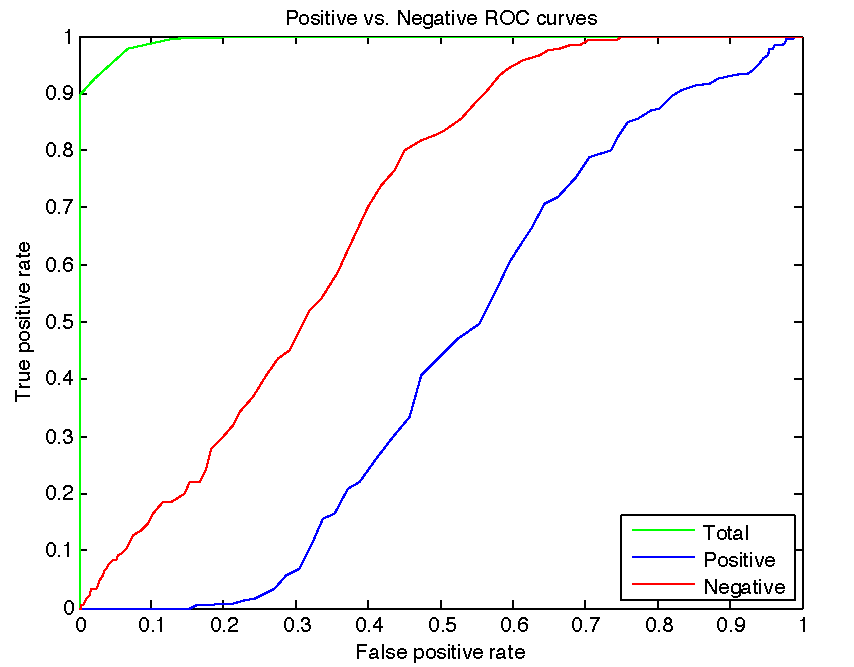
\includegraphics[width=3in]{roc_pos_vs_neg}
\caption{Comparison of positive and negative ROC curves. From left to right: the first curve (green) refers to a classifier that uses the total reconstruction error (eq. \ref{total_error}) and has an AUC of 0.995; the second curve (red) refers to a classifier that uses only the reconstruction errors from negative PCs ($d_{gn}$ and $d_{en}$) and has an AUC of 0.690; and the third curve (blue) refers to a classifier that uses only the errors from positive PCs ($d_{gp}$ and $d_{ep}$) and has an AUC of 0.444. On the three classifiers, only the first 100 principal components are being used, that is, $k=100$. Both positive and negative classifiers yields a poor result, far from the full classifier performance. It is surprising to see that the negative classifier even got a better result than the positive one.}
\label{roc_pos_vs_neg}
\end{figure}

To understand why this happens, it is interesting to see how the reconstruction errors are distributed. In Figure~\ref{dist_pos_vs_neg}, we plot the reconstruction error of each individual test sample in the three situations previously described. It is possible to see that the samples are mixed on the two first plots, indicating that these criteria do not have discriminatory power to correctly separate the samples. Conversely, when the errors are combined, the distribution changes completely and we can notice that samples from different classes are in fact grouped, what makes possible the high classification accuracy we got. Hence, the reconstruction errors from both positive and negative PCs contribute in a significant way to the classification and none of them can be removed.

\begin{figure}[t!]
\centering
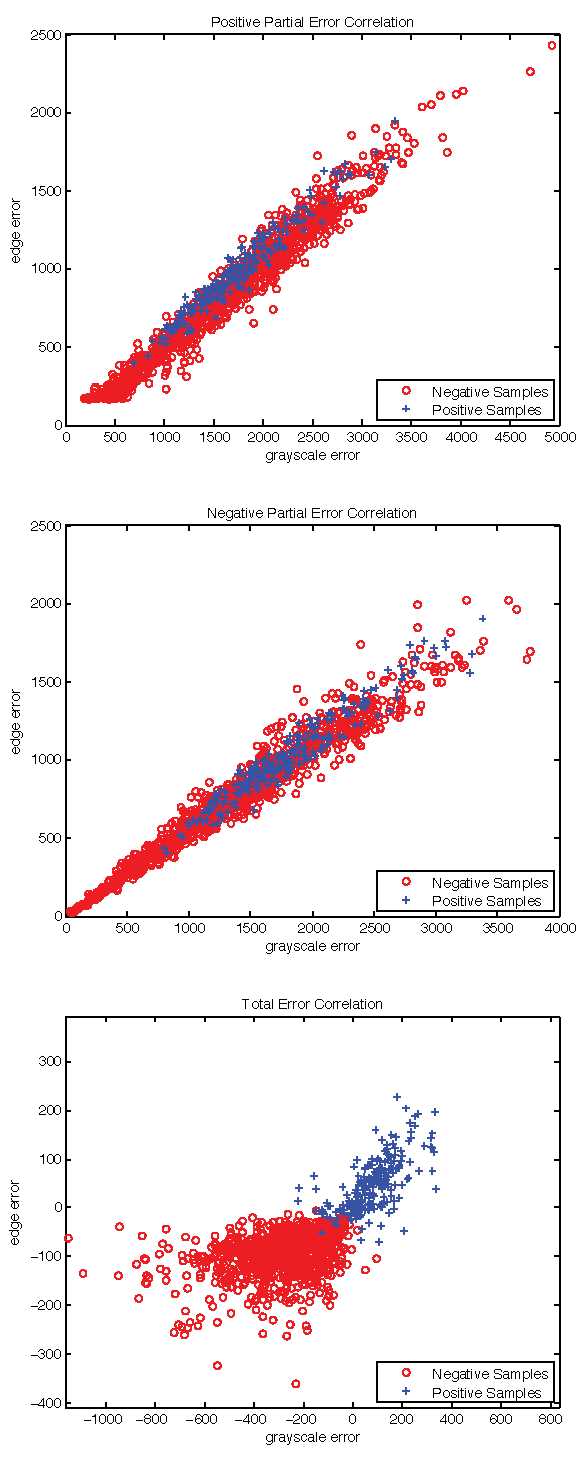
\includegraphics[width=3in]{dist_pos_vs_neg}
\caption{Comparison of reconstruction errors distributions. The first chart plots the errors of test samples when only the reconstructions from positive PCs are being considered. The second chart plots the errors only for the negative reconstructions. And the third chart plots the distribution of the total reconstruction error. Note that the errors are mixed on the first two charts; classify the samples based on them is a hard task. On the other hand, the third chart show well defined clusters of errors, what makes possible a good classification. This explains the curves of Figure~\ref{roc_pos_vs_neg}.}
\label{dist_pos_vs_neg}
\end{figure}

On the other hand, we get very similar ROC curves when the classifier considers the reconstruction errors from grayscale PCs and from edge PCs separately (now always using the errors from positive PCs and from negative PCs together). This in shown in Figure~\ref{roc_gray_vs_edge}, which exhibit three ROC curves: one from the classifier that uses only grayscale errors, one from the classifier that uses only edge errors and one from the classifier that considers both (i.e. the total reconstruction error). Note that the ROC curves from the edge error classifier and from the total error classifier are nearly indistinguishable. In fact, their area under the curve (AUC) are practically equal.

\begin{figure}[t!]
\centering
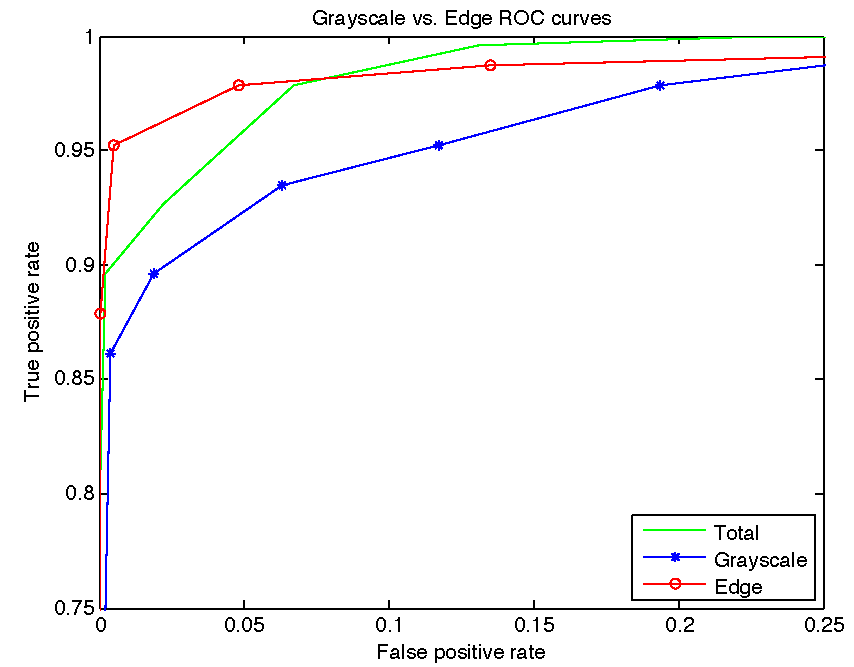
\includegraphics[width=3in]{roc_gray_vs_edge}
\caption{Comparison of grayscale and edge ROC curves. The green curve refers to a classifier that uses the total reconstruction error (eq. \ref{total_error}) and has an AUC of 0.995; the red curve refers to a classifier that uses only the reconstruction errors from edge PCs ($d_{ep}$ and $d_{en}$) and has an AUC of 0.994; and the blue curve uses only the errors from grayscale PCs ($d_{gp}$ and $d_{gn}$) and has an AUC of 0.985. On the three classifiers, only the first 100 principal components are being used, that is, $k=100$. Note that the scale is different of that from Figure~\ref{roc_pos_vs_neg}; we approximated the upper left corner to better show the small difference between the curves.}
\label{roc_gray_vs_edge}
\end{figure}

Again, we plot the reconstruction error distributions, but now segregating errors from grayscale PCs and from edges PCs. These plots are shown in Figure~\ref{dist_gray_vs_edge}, that also displays a plot of the total reconstruction error. Now, we get a different scenario. All the three plots exhibit a clear boundary that separate samples from different classes. This indicate that there is a lot of redundancy between errors from grayscale PCs and from edge PCs and one of them can be safely removed from the classifier with just a minor impact on the classification accuracy. Our results indicate that the errors from grayscale PCs generally yields a slightly worse result, as shown in the Table~\ref{table_gray_vs_edge}. Therefore, it is possible to compose a classifier only with the edge errors and speed up the classification significantly (since two reconstructions will not have to be computed anymore). In general, such classifier drops the classification accuracy in less than $1\%$ when compared with a classifier that uses the total error. Actually, the classifier based only on the edge errors sometimes performs even better than the full classifier in our experiments (when $k >= 200$), as also shown in Table~\ref{table_gray_vs_edge}.

\begin{figure}[tl!]
\centering
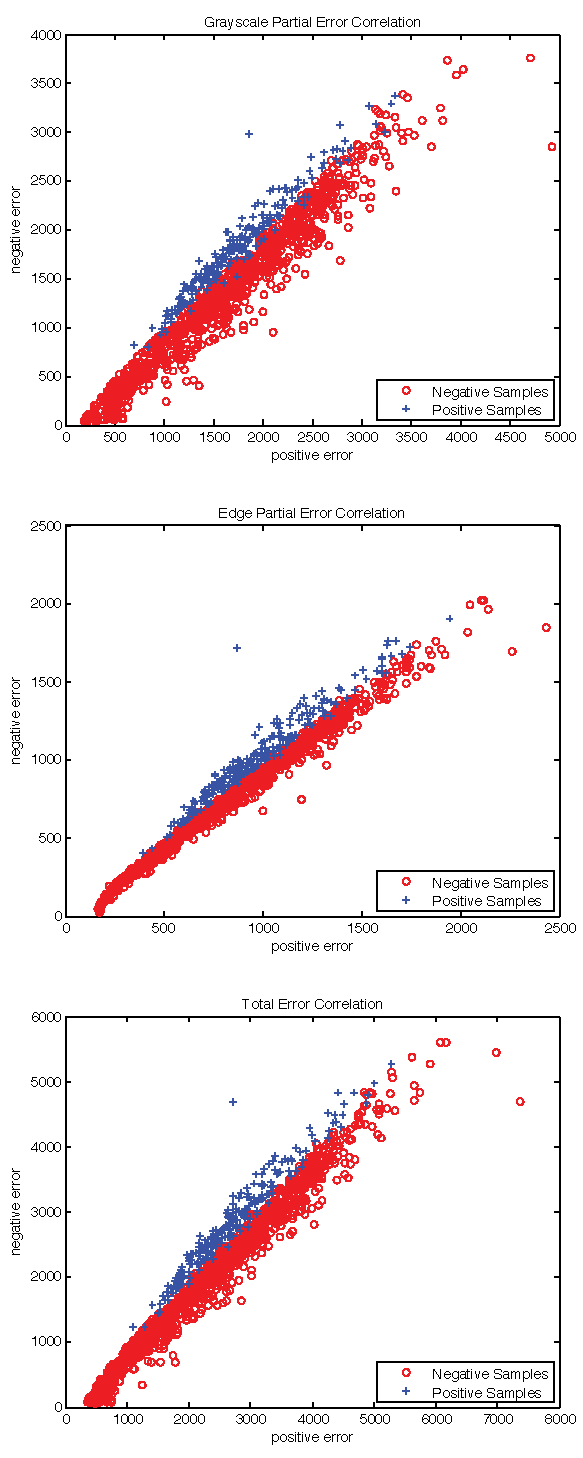
\includegraphics[width=3in]{dist_gray_vs_edge}
\caption{Comparison of reconstruction errors distributions. The first chart plots the errors of positive and negative test samples when only the reconstructions from grayscale PCs are being considered. The second chart plots the errors only for the edge reconstructions. And the third chart plots the distribution of the total reconstruction error. Note that the three charts show a clear boundary between errors from positive and from negative samples.}
\label{dist_gray_vs_edge}
\end{figure}

\begin{table}[t]
  \caption{AUCs for grayscale, edge and total errors classifiers}
  %{Comparison of area under the curve (AUC) of the classifiers based on grayscale error, edge error, and total error, respectively, for many values of $k$. The AUCs of the edge-based classifier are always larger then the grayscale-based classifier. This indicates edge errors are more relevant to the classification.}
  \begin{center}
    \begin{tabular}{  c | c  c  c  }
      \hline
      $k$ & Gray & Edge & Total \\
      \hline
      400 & 0.9611 & 0.9863 & 0.9744 \\
      300 & 0.9694 & 0.9877 & 0.9826 \\ 
      200 & 0.9768 & 0.9905 & 0.9877 \\
      100 & 0.9851 & 0.9944 & 0.9948 \\
      50  & 0.9905 & 0.9956 & 0.9972 \\
      25  & 0.9929 & 0.9913 & 0.9984 \\
      \hline  
    \end{tabular}
  \end{center}
  \label{table_gray_vs_edge}
\end{table}

% What reference use to GA?
These findings point out that, among the four reconstruction errors, some are more relevant to the classification than others. However, on the total reconstruction error (eq. \ref{total_error}) each error contributes equally. Thus, we use the weighted total reconstruction error (eq. \ref{weighted_total_error}) to improve the classification accuracy. The problem with using weights is how to choose them. We can try some values and make adjustments manually, test after test. But we can also employ an optimization algorithm that looks for the values in an automated way. In this work, we use a genetic algorithm~\cite{goldberg89}. It initially chooses a set of random values and uses operations as crossover and mutation to improve them during many iterations. The values are adjusted in relation to a fitness function. In our case, this functions aims to correctly classify the largest number of training samples using a given set of weights. The function can be fine-tuned in order to give more importance in finding more pedestrians despite the false detections or to minimize the number of non-pedestrians classified as pedestrians.

As this algorithm performs a local optimization and therefore is not optimum, we runned it five times for each value of $k$. We then have chosen the set of weights that gets the best classification rates among these five. Finally, we classify the test samples considering the weighted total reconstruction error. The produced ROC curves always have a larger AUC than the corresponding versions without weights for all values of $k$ we tested. This is shown in Figure~\ref{auc_vs_k}. The difference is more pronounced for large values of $k$ and becomes small when $k$ diminishes. Still, the AUC of the weighted classifier is always larger, what indicates that the weighted error is a better classification criteria than the non-weighted one. Finally, we plotted the distribution of the weighted total reconstruction error, that can be seen in Figure~\ref{dist_weighted}. This time, we get a clear boundary between errors from samples of different classes.

\begin{figure}[t]
\centering
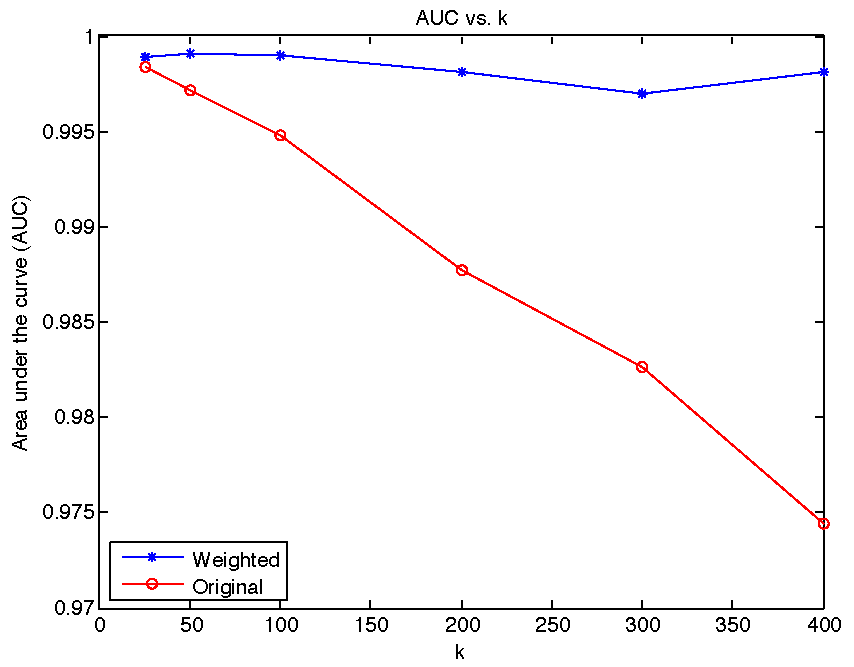
\includegraphics[width=3in]{chart_auc_vs_k}
\caption{Comparison of weighted and original classifiers AUCs for different values of $k$. The AUCs of the weighted classifier are more stable when $k$ varies.}
\label{auc_vs_k}
\end{figure}

\begin{figure}[t]
\centering
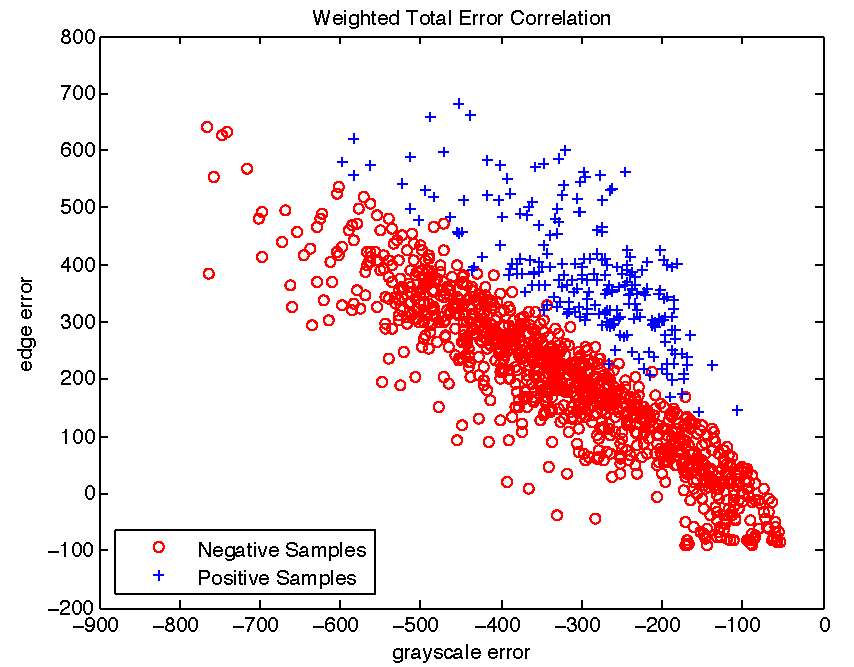
\includegraphics[width=3in]{dist_gray_vs_edge_weighted}
\caption{Distribution of the weighted total reconstruction errors for positive and for negative training samples, for $k=100$. Compare it with the third chart of Figure~\ref{dist_pos_vs_neg}. Here the boundary between errors from positive and from negative samples is much clearer.}
\label{dist_weighted}
\end{figure}

% The better value of k depends on the particular application

% \begin{table}
%   \caption{Selected weights}
%   %{Weights that produced best classification rates for each value of $k$. Note that the weights associated to edge errors are usually larger than the errors associated to grayscale errors, what reinforces the greater importance of the edge errors to the classification.}
%   \begin{center}
%     \begin{tabular}{  c | c  c  c  c  }
%       \hline
%       $k$ & $w_{gp}$ & $w_{ep}$ & $w_{gn}$ & $w_{en}$ \\
%       \hline
%       400 & 0.4456 & 0.5472 & 0.2785 & 0.9340 \\
%       300 & 1.6523 & 0.7827 & 0.9183 & 2.2065 \\
%       200 & 0.3101 & 0.6551 & 0.1338 & 0.9962 \\
%       100 & 0.8472 & 1.3322 & 0.7671 & 1.5308 \\
%       50  & 0.2236 & 0.8294 & 0.1905 & 0.9043 \\
%       25  & 0.9172 & 1.1696 & 0.7768 & 1.4662 \\
%       \hline  
%     \end{tabular}
%   \end{center}
%   \label{table_weights}
% \end{table}

% k pgp pep pgn pen Total AUC Weighted AUC
% 400 0.4456  0.5472  0.2785  0.9340  0.9744  0.9981
% 300 1.6523  0.7827  0.9183  2.2065  0.9826  0.9970
% 200 0.3101  0.6551  0.1338  0.9962  0.9877  0.9981
% 100 0.8472  1.3322  0.7671  1.5308  0.9948  0.9990
% 50  0.2236  0.8294  0.1905  0.9043  0.9972  0.9991
% 25  0.9172  1.1696  0.7768  1.4662  0.9984  0.9989

% TODO Figure with k vs AUC for non-weighted and weighted


% An example of a floating figure using the graphicx package.
% Note that \label must occur AFTER (or within) \caption.
% For figures, \caption should occur after the \includegraphics.
% Note that IEEEtran v1.7 and later has special internal code that
% is designed to preserve the operation of \label within \caption
% even when the captionsoff option is in effect. However, because
% of issues like this, it may be the safest practice to put all your
% \label just after \caption rather than within \caption{}.
%
% Reminder: the "draftcls" or "draftclsnofoot", not "draft", class
% option should be used if it is desired that the figures are to be
% displayed while in draft mode.
%
%\begin{figure}[!t]
%\centering
%\includegraphics[width=2.5in]{myfigure}
% where an .eps filename suffix will be assumed under latex, 
% and a .pdf suffix will be assumed for pdflatex; or what has been declared
% via \DeclareGraphicsExtensions.
%\caption{Simulation Results}
%\label{fig_sim}
%\end{figure}

% Note that IEEE typically puts floats only at the top, even when this
% results in a large percentage of a column being occupied by floats.


% An example of a double column floating figure using two subfigures.
% (The subfig.sty package must be loaded for this to work.)
% The subfigure \label commands are set within each subfloat command, the
% \label for the overall figure must come after \caption.
% \hfil must be used as a separator to get equal spacing.
% The subfigure.sty package works much the same way, except \subfigure is
% used instead of \subfloat.
%
%\begin{figure*}[!t]
%\centerline{\subfloat[Case I]\includegraphics[width=2.5in]{subfigcase1}%
%\label{fig_first_case}}
%\hfil
%\subfloat[Case II]{\includegraphics[width=2.5in]{subfigcase2}%
%\label{fig_second_case}}}
%\caption{Simulation results}
%\label{fig_sim}
%\end{figure*}
%
% Note that often IEEE papers with subfigures do not employ subfigure
% captions (using the optional argument to \subfloat), but instead will
% reference/describe all of them (a), (b), etc., within the main caption.


% An example of a floating table. Note that, for IEEE style tables, the 
% \caption command should come BEFORE the table. Table text will default to
% \footnotesize as IEEE normally uses this smaller font for tables.
% The \label must come after \caption as always.
%
%\begin{table}[!t]
%% increase table row spacing, adjust to taste
%\renewcommand{\arraystretch}{1.3}
% if using array.sty, it might be a good idea to tweak the value of
% \extrarowheight as needed to properly center the text within the cells
%\caption{An Example of a Table}
%\label{table_example}
%\centering
%% Some packages, such as MDW tools, offer better commands for making tables
%% than the plain LaTeX2e2e tabular which is used here.
%\begin{tabular}{|c||c|}
%\hline
%One & Two\\
%\hline
%Three & Four\\
%\hline
%\end{tabular}
%\end{table}


% Note that IEEE does not put floats in the very first column - or typically
% anywhere on the first page for that matter. Also, in-text middle ("here")
% positioning is not used. Most IEEE journals/conferences use top floats
% exclusively. Note that, LaTeX2e, unlike IEEE journals/conferences, places
% footnotes above bottom floats. This can be corrected via the \fnbelowfloat
% command of the stfloats package.



\section{Conclusion}

In this work we analyzed a classifier that uses PCA image reconstruction for pedestrian detection. It uses four sets of principal components (PCs): two originated from grayscale and edge images that contains pedestrians, respectively, and two originated from grayscale and edge images that did not contain pedestrians, respectively. To classify an image, it uses these sets of PCs to perform four image reconstructions and compares the respective reconstruction errors to determine if the given image depicts or not a pedestrian.

To understand how the individual errors contribute to the overall performance, we compared two classifiers: one that uses only the reconstructions from the positive PCs and other that uses only the reconstructions from the negative PCs. In our experiments, both performed poorly when compared to the full classifier, indicating that positives and negatives reconstructions are indeed relevant to the classification. The crucial role of the reconstructions from negative PCs is particularly surprising, since non-pedestrian samples are not related and do not contain a specific pattern. Therefore, we conclude that the importance of the negative reconstructions is not on what they characterize, but instead on what they do not characterize. In this way, the negative reconstruction errors contribute to raise the total reconstruction error when the image does not contain a pedestrian, what makes possible a better classification.

We also investigated the relevance of grayscale and edge errors. In other experiment we compared the accuracy of a classifier that uses only grayscale reconstructions and other classifier that uses only edge reconstructions. This time, they performed very well, with a performance close to that of the total error classifier. This suggest that there is a lot of redundancy between grayscale and edge information. The classifier based only on edge images got better results, indicating that edge information is more relevant to this classifier. In fact, the edge classifier performed better than the total error classifier itself in some cases and, when the results were worse, the accuracy drop was less than 1\%. For this reason, it is possible to speed up the classification time in a significant way by using only edge information and keep the classification accuracy virtually unchanged.

Since our experiments show that each error has a different relevance for classification, we propose a classifier that uses a weighted version of the total reconstruction error. The problem with weights, though, is how to find the best values. To get an approximation in an automated way, we used a genetic algorithm with a fitness function that aims to achieve the best classification rates for the training samples. This classified performed better than the original version in our experiments for all numbers of PCs we tested. % DESCRIBE CLASSIFICATION RATE VS K

% Future work include testing this classifier with other pedestrian databases and verifying if the reconstruction approach is suitable to other detection problems in computer vision, such as face detection. We intend to develop the classifier into a complete detection system, capable of locate objects in large pictures.% It is also possible to employ variations of PCA for reconstruction, like the more robust 2D-PCA \cite{li05}.


% The dimensions affect not in a linear way, e.g., the more the better is wrong.

% conference papers do not normally have an appendix


% use section* for acknowledgement
% \section*{Acknowledgment}
% 
% 
% The authors would like to thank...
% more thanks here


% trigger a \newpage just before the given reference
% number - used to balance the columns on the last page
% adjust value as needed - may need to be readjusted if
% the document is modified later
%\IEEEtriggeratref{8}
% The "triggered" command can be changed if desired:
%\IEEEtriggercmd{\enlargethispage{-5in}}

% references section

% can use a bibliography generated by BibTeX as a .bbl file
% BibTeX documentation can be easily obtained at:
% http://www.ctan.org/tex-archive/biblio/bibtex/contrib/doc/
% The IEEEtran BibTeX style support page is at:
% http://www.michaelshell.org/tex/ieeetran/bibtex/
\bibliographystyle{IEEEtran}
% argument is your BibTeX string definitions and bibliography database(s)
\bibliography{paper}
%
% <OR> manually copy in the resultant .bbl file
% set second argument of \begin to the number of references
% (used to reserve space for the reference number labels box)
%\begin{thebibliography}{1}

%\bibitem{IEEEhowto:kopka}
%H.~Kopka and P.~W. Daly, \emph{A Guide to \LaTeX}, 3rd~ed.\hskip 1em plus
%  0.5em minus 0.4em\relax Harlow, England: Addison-Wesley, 1999.

%\end{thebibliography}




% that's all folks
\end{document}